\documentclass{exam}

\usepackage[top=0.9in, bottom=1in, left=1.5in, right=1.5in]{geometry}
\usepackage[utf8]{inputenc}
\usepackage[icelandic]{babel}
\usepackage[T1]{fontenc}
\usepackage[sc]{mathpazo}

\usepackage[parfill]{parskip}
\usepackage{booktabs,tabularx}
\usepackage{multirow}
\usepackage{enumerate}
\usepackage{graphicx}
\usepackage{amsmath, amsfonts, amssymb, amsthm}
\usepackage{tikz}
\makeatletter % Fix due to (recent versions of?) minted containing their own framed definition
\expandafter\providecommand\expandafter*\csname ver@framed.sty\endcsname
{2003/07/21 v0.8a Simulated by exam}
\makeatother
\usepackage{minted} %Minted and configuration

\usepackage[pdftex,bookmarks=true,colorlinks=true,pdfauthor={Eirikur Ernir Thorsteinsson},linkcolor=blue,urlcolor=blue]{hyperref}

\setcounter{secnumdepth}{-1} 
\hyphenpenalty=5000


% Picture locations
\graphicspath{{./Pics/}}

\usemintedstyle{default}
\renewcommand{\theFancyVerbLine}{\sffamily \arabic{FancyVerbLine}}

\newcommand{\Mod}[1]{\ \text{mod}\ #1}

\runningfooter{\hspace{-2cm}
\includegraphics[width=0.5\textwidth]{Pics/hi-von-logo}}{}{}

\renewcommand{\solutiontitle}{\noindent\textbf{Mögulegt svar:}}

\author{}
\date{}

\footer{}{}{}

\usepackage{graphicx}
\usepackage{caption}
\usepackage{subcaption}

\title{Stærðfræðimynstur í tölvunarfræði \\ Skilaverkefni 9}
\author{}

\printanswers

\begin{document}
\maketitle
\thispagestyle{empty} 

Skila skal þessu verkefni á vefnum \href{https://gradescope.com/}{Gradescope}. Aðgangskóði fyrir námskeiðið er \textbf{926WD9}.


\section{Spurningar}

\begin{questions}

\section{Kaflar 10.1 og 10.2}

\question Lítum á óstefnt net sem táknar samfélagstengsl, eins og t.d. eftirfarandi net:

\begin{center}
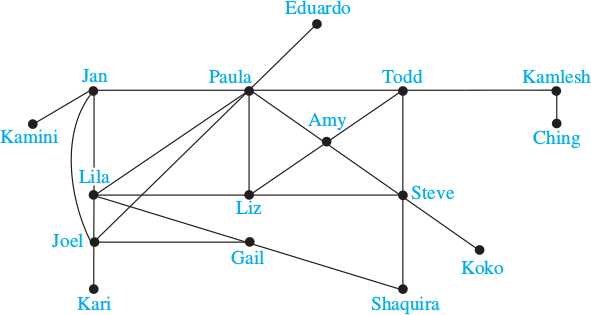
\includegraphics[width=0.5\textwidth]{acquaintanceship}
\end{center}

Gerum ráð fyrir að við séum með net af þessu tagi sem táknar gagnkvæman kunningsskap alls fólks í heiminum. Hvað táknar stig hnúts í slíku neti? Hvað tákna hnútar af stigi 0? Hvað táknar nágrannamengi hnúts? Hvað táknar það að meðalstig hnúta í þessu neti sé 1000?

\paragraph{Í bók:} Exercise 10.2.12

\question 

\textbf{(Ísl)} Látum $G$ vera óstefnt net með 5 hnútum. Er mögulegt að eftirfarandi talnarunur séu listar yfir stig hnútanna í $G$? Teiknaðu $G$ í þeim tilvikum þar sem það er hægt.

\textbf{(En)} Let $G$ be an undirected graph with 5 vertices. Is it possible that the following sequences form a list of the degrees of $G$'s vertices? Where possible, draw $G$.

\begin{enumerate}[a)]
\item $1,2,2,3,4$
\item $2,2,4,4,4$
\item $4,4,4,4,4$
\item $1,2,2,3,5$
\end{enumerate}

\paragraph{Í bók:} Þetta dæmi er ekki í bókinni.

\newpage

\begin{enumerate}
 \item  Mögulegt. Sjá mynd.
 \item  Mögulegt. Sjá mynd.
 \item  Mögulegt. Sjá mynd.
 \item  Ekki mögulegt. Sjá setningu um fjölda hnúta af oddatölustigi.
\end{enumerate}

\begin{figure}[hb]
\caption{Möguleg net}
\label{mynd:verkefni3}
\centering
\begin{subfigure}[b]{0.3\textwidth}
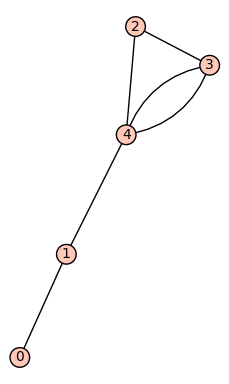
\includegraphics[width=\textwidth]{Skil9a}
\caption{Net með hnútum af stigum $1,2,2,3$ og $4$}
\end{subfigure}
\hspace{0.5cm}
\begin{subfigure}[b]{0.3\textwidth}
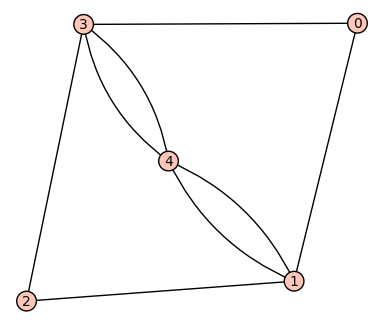
\includegraphics[width=\textwidth]{Skil9b}
\caption{Net með hnútum af stigum $2,2,4,4$ og $4$}
\end{subfigure}
\hspace{0.5cm}
\begin{subfigure}[b]{0.3\textwidth}
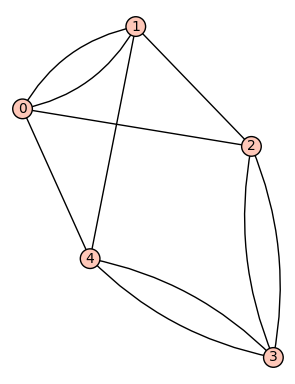
\includegraphics[width=\textwidth]{Skil9c}
\caption{Net með hnútum af stigum $4,4,4,4$ og $4$}
\end{subfigure}
\end{figure}

\question Sýnið að óstefnt, einfalt net $G$ sem inniheldur að minnsta kosti tvo hnúta hafi að minnsta kosti tvo hnúta af sama stigi.

\paragraph{Í bók:} Exercise 10.2.18

\question Fyrirtæki nokkurt hefur fimm manneskjur á starfsmannaskrá: Zamora, Agraharam, Smith, Chou og Jónatan. Hvert þeirra mun sinna einu af sex mögulegum störfum, sem eru: skipulagning, almannatengsl, sölustjórn, markaðsstjórn, þróun og atvinnulífstengsl. Zamora getur sinnt skipulagningu, sölustjórn, markaðsstjórn eða atvinnulífstengslum. Agraharam getur sinnt skipulagning eða þróun. Smith getur sinnt almannatengslum, sölustjórn eða atvinnulífstengslum. Chou getur sinnt skipulagningu, sölustjórn eða atvinnulífstengslum. Jónatan getur sinnt skipulagningu, almannatengslum, sölustjórn eða atvinnulífstengslum.

\begin{enumerate}[a)]
 \item Settu hæfileika þessa starfsfólks fram með því að nota tvíhlutanet
 \item Deildu út störfum meðal starfsfólksins svo að hvert þeirra hafi nákvæmlega eitt starfssvið
 \item Er spyrðingin sem samsvarar útdeilingunni í lið b) fullkomin spyrðing frá mengi starfsfólks til mengis starfa? Er spyrðingin af hámarksstærð?
\end{enumerate}

\paragraph{Í bók:} Exercise 10.2.28

\section{Kafli 10.3}

\question Teiknaðu netið sem hefur eftirfarandi grennslafylki:

\[
\begin{bmatrix}
1&1&1&0\\
0&0&1&0\\
1&0&1&0\\
1&1&1&0\\
\end{bmatrix}
\]

\paragraph{Í bók:} Exercise 10.3.12

\question Settu fram grennslafylki fyrir eftirfarandi net:

\begin{enumerate}[a)]
 \item Fullskipaða netið $K_n$
 \item Hjólið $W_n$
\end{enumerate}

\paragraph{Í bók:} Hluti af exercise 10.3.32



\end{questions}


\end{document}